\section{Federated Learning}
% Types of Federated Learning:
% \begin{enumerate}
%     \item Cross-device. (1) Huge \#sources, (2) each with small amount of data, (3) dynamically drop in and out in the learning process, (4) contact rarely. Example: Google spell checker.
%     \item Cross-sillo. (1) Limited \#sources, (2) each with a lot of data, (3) participate constantly, (4) potentially heterogeneous. Example: Hospitals MRI segmentation.
% \end{enumerate}
Communication Round: (1) Server selects clients to participate. (2) Clients do local training update on private data and send information to the server. (3) Server aggregates updates into updated model.

\subsection*{FedSGD}
Clients compute gradient wrt. (minibatch of) local data on global weights. Server takes average for global update. Pros: convergence guarantee. Cons: requires lots of communication. Gradient inversion:
\begin{center}
    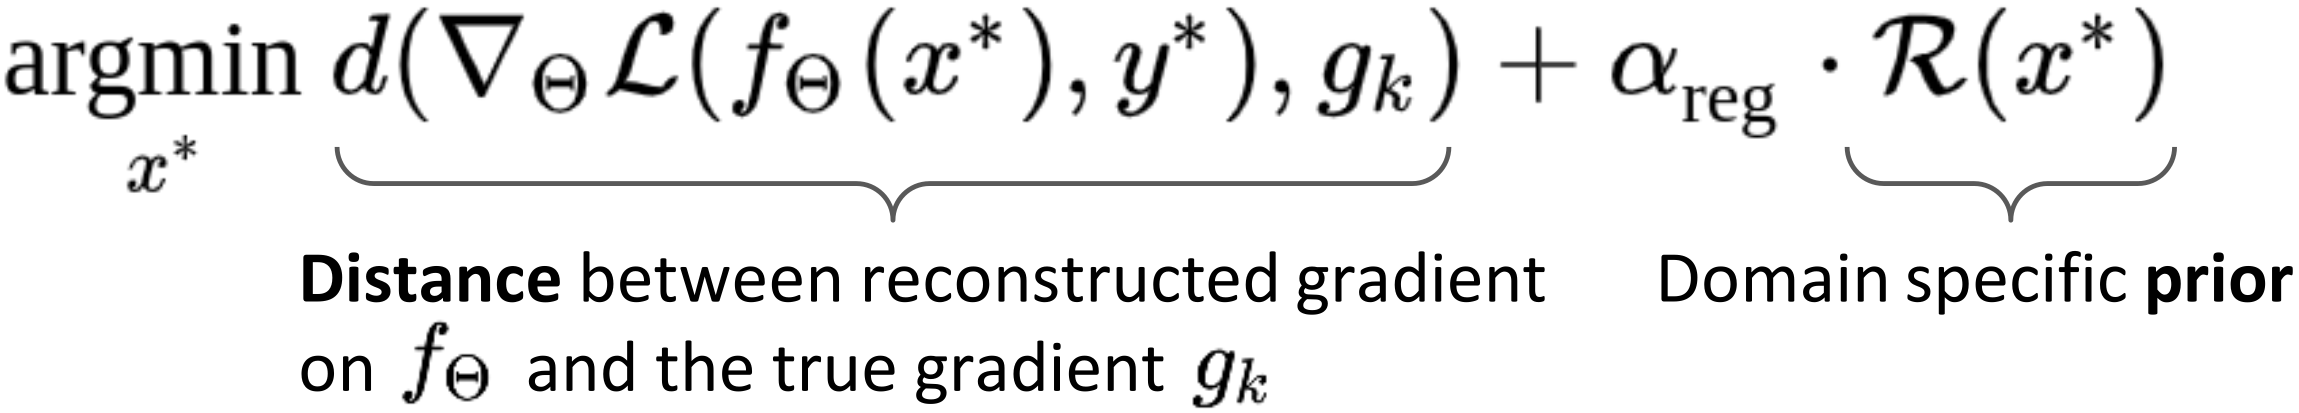
\includegraphics[width=0.7\linewidth]{img/gradient_inversion.png}
\end{center}
% \vspace*{-3mm}

\subsection*{FedAvg} Do several iterations of local SGD on the global weights and average the local weights as the global weight. Pros: Less communication. Cons: No convergence guarantee.

% \subsection*{Issues}
% \begin{itemize}
%     \item Honest-but-Curious Server: honestly follow the algorithm but want to expose private data of clients. Gradient inversion: match gradients of reconstructed and client data.
%     \item Client-side poisoning: send crafted updates to the server to force divergence or bad behavior on certain data.
%     \item Client fairness: model behaves well on average but poorly for certain clients due to heterogeneity. There is a trade-off between preventing client-side poisoning and client fairness because the server cannot tell whether a bad update is malicious or because of heterogeneity.
% \end{itemize}